\documentclass{article}

\textwidth=6.5in
\textheight=8.5in
\voffset=-54pt
\oddsidemargin=0in
\evensidemargin=0in
\setlength{\parskip}{8pt}
\setlength{\parindent}{0pt}

\usepackage{workbook}

\usepackage{handout}

\usepackage{exam}

\newcommand{\answerbox}[3][]{
    \fbox{\begin{minipage}[t][#2][c]{#3}
        Final answer: #1
    \end{minipage}}
    }
    
\begin{document}

 

 \noindent
{\large \mbox{} \hfill \bf Name:\underline{\hspace{2.8in}}}

 {\mbox{} \hfill \it (Please write your name neatly in print.)}


 
\medskip
 
\noindent
{\large\bf
Practice Integration Skills Check 1 \\ Math Mb Spring 2025}
\noindent






\iffalse
\begin{center}
\begin{tabular}{|c|c|c|}
\hline
Problem & Points & Score\\ \hline
& &\\
1 &  & \\ 
\hline
&& \\
2&  &  \\ 
\hline
& &\\
3&&  \\ 
 \hline
& &\\
Total&  &  \\ 
& &\\ \hline

\end{tabular}
\end{center}
\fi


{\Large
\begin{center}\textbf{Directions---Please read carefully!} \end{center}}

This is a practice test. The same directions will appear on the actual Skills Check, so read them carefully.

\hrulefill 

You have 60 minutes to complete this Skills Check. \textbf{Calculators or any other aids are not permitted.}  


For each problem, write your final answer in the answer box provided. You may do work on any page and may ask for scratch paper, but \textbf{no work or writing outside of the answer box will be graded.}

Write neatly, as answers that cannot be read will not receive credit. 

   

\begin{center}\textbf{Good luck!}\end{center}


\newpage

\begin{enumerate}

\item Find the following basic \textbf{indefinite} integrals.

\begin{enumerate}
    \item $\displaystyle \int x^n \;dx$ (for $n \neq -1$)
    \vfill 
    \answerbox[\solonly{$\frac{1}{n+1}x^{n+1}+C$}]{.5 in}{5.5 in}
    
    \item $\displaystyle \int \sin(x) \;dx$
    \vfill 
    \answerbox[\solonly{$-\cos(x)+C$}]{.5 in}{5.5 in}
    
    \item $\displaystyle \int e^x \;dx$
    \vfill 
    \answerbox[\solonly{$e^x+C$}]{.5 in}{5.5 in}

    \item $\displaystyle \int \frac{1}{1+x^2} \;dx$
    \vfill 
    \answerbox[\solonly{$\arctan(x) +C$}]{.5 in}{5.5 in}
    
    \item $\displaystyle \int \frac{1}{x}\;dx $
    \vfill 
    \answerbox[\solonly{$\ln\!|x|+C$}]{.5 in}{5.5 in}
    
    \item $\displaystyle \int \cos(x)\;dx$
    \vfill 
    \answerbox[\solonly{$\sin(x)+C$}]{.5 in}{5.5 in}

\end{enumerate}

\newpage 



\item Find each integral. You may use any method. \textbf{Fully simplify your answers to all definite integrals.}
\begin{enumerate}

          
    \item $ \displaystyle \int \tan(t) \;dt$
    \vfill 
    \answerbox[\solonly{$-\ln\!|\cos(t)|+C$}]{.5 in}{5.5 in}

    \item $\displaystyle \int_0^{\pi} \sin(x) \;dx$
    \vfill 
    \answerbox[\solonly{$2$}]{.5 in}{5.5 in}

    \item $\displaystyle \int (6t^5 - 12t^3 + 5t + 2)\;dt$
    \vfill 
    \answerbox[\solonly{$t^6-3t^4+\frac{5}{2}t^2+2t+C$}]{.5 in}{5.5 in}
    
    \newpage 
    
    \item $ \displaystyle \int_0^2 \sqrt{4-x^2} \; dx$
    \vfill 
    \answerbox[\solonly{$\pi$}]{.5 in}{5.5 in}
    
    \item $\displaystyle \int \frac{x^3 +2x^2-x}{x^2} \;dx$
    \vfill 
    \answerbox[\solonly{$\frac{1}{2}x^2+2x-\ln\!|x|+C$}]{.5 in}{5.5 in}

    \newpage 
    
    \item $\displaystyle \int x \sin(x^2)\;dx$
    \vfill 
    \answerbox[\solonly{$-\frac{1}{2}\cos(x^2)+C$}]{.5 in}{5.5 in}
    
    \item $\displaystyle \int \ln(t)\;dt$
    \vfill 
    \answerbox[\solonly{$t\ln(t) - t +C$}]{.5 in}{5.5 in}

\newpage 

    \item $\displaystyle \int u \sqrt{u-3} \;du$
    \vfill 
    \answerbox[\solonly{$\frac{2}{5}(u-3)^{5/2}+2(u-3)^{3/2}+C$}]{.5 in}{5.5 in}

    \item $\displaystyle \int_{\frac{\pi}{2}}^{\frac{3\pi}{2}} x \cos(x) \;dx$
    \vfill 
    \answerbox[\solonly{$-2\pi$}]{.5 in}{5.5 in}

\end{enumerate}

\newpage 

\item We want to approximate the area of the region $\mathcal{R}$ shown below using a right Riemann sum with 100 equal sub-intervals, $R_{100}$. $\mathcal{R}$ is bounded by the curves $y=f(x)$, $y=0$, $x=1$, and $x=2$, where $f(x)=e^x$.

    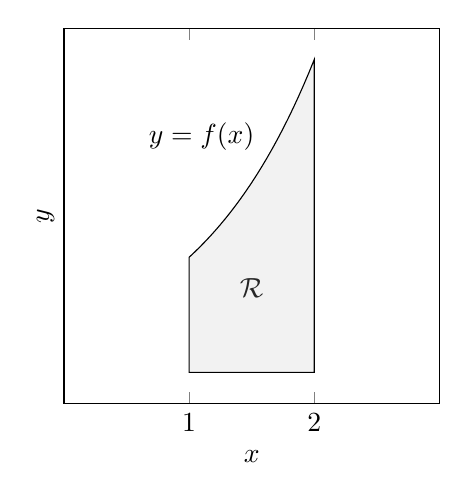
\begin{tikzpicture} 
      \begin{axis}[stack plots=y, cycle list={black}, xmin=0, xmax=3, 
        width=2.5in, height=2.5in, clip=false, ytick=\empty,
        xtick={1,2}, xlabel=$x$, ylabel=$y$] 
        \addplot+[domain=1:2]{0} node [right] {\;} ; 
        \addplot+[domain=1:2, fill=lightgray, fill opacity=0.2] 
        {e^x} \closedcycle; 
        \node [above] at (axis cs: 1.1, 5) {$y=f(x)$};
        \node at (axis cs:1.5, 2) {$\mathcal{R}$};
              \end{axis} 
    \end{tikzpicture}
\begin{enumerate}
    \item Write down the value of $\Delta x$.
    \vfill
    \answerbox[$\Delta x =\solonly{\frac{1}{100}}$]{.5 in}{5.5 in}
    \item Write down a formula for $x_k$, the right endpoint of the $k$th sub-interval.
    \vfill
    
    \answerbox[$x_k=\solonly{1+\frac{1}{100}k}$]{.5 in}{5.5 in}
    \item Write down a formula for $R_{100}$ using sigma notation. 
    \vfill
    
    \answerbox[$R_{100}=\solonly{\displaystyle\sum_{k=1}^{100} e^{x_k}\Delta x}$\solonly{ or $R_{100}=\displaystyle\sum_{k=1}^{100} \tfrac{1}{100}e^{1+k/100}$}]{.75 in}{5.5 in}
\end{enumerate}
    
    
\end{enumerate}


\end{document}